% To convert to svg
% lualatex --output-format=dvi mother.tex
% dvisvgm mother.dvi
\documentclass[dvisvgm]{minimal}		%uncomment to convert to svg

% \documentclass[border=0]{standalone}
\usepackage{tikz}
\usetikzlibrary {shapes.geometric}
\usepackage{xcolor}
\definecolor{highlight2}{HTML}{99cc99}
\begin{document}
    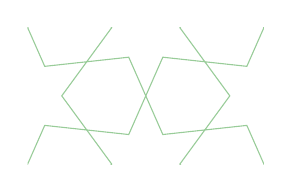
\begin{tikzpicture}
        \pgfmathsetmacro{\a}{sqrt(3)}
        \pgfmathsetmacro{\b}{\a/4}
        \clip (0.5,0) rectangle (3.5,-\a);
        \node [star,star points=6, star point height=\b cm, minimum size=\a cm, draw,highlight2] at (2,0) {};    
        \node [star,star points=6, star point height=\b cm, minimum size=\a cm, draw,highlight2] at (2,{-sqrt(3)}) {};    
        \node [star,star points=6, star point height=\b cm, minimum size=\a cm, draw,highlight2] at (1/2,{-sqrt(3)/2}) {};    
        \node [star,star points=6, star point height=\b cm, minimum size=\a cm, draw,highlight2] at (1/2,{sqrt(3)/2}) {};    
        \node [star,star points=6, star point height=\b cm, minimum size=\a cm, draw,highlight2] at (7/2,{sqrt(3)/2}) {};    
        \node [star,star points=6, star point height=\b cm, minimum size=\a cm, draw,highlight2] at (7/2,{-sqrt(3)/2}) {};    
    \end{tikzpicture}
\end{document}
